\documentclass{sig-alternate}
  \pdfpagewidth=8.5truein
  \pdfpageheight=11truein


%\clubpenalty=10000
%\widowpenalty = 10000

\newfont{\mycrnotice}{ptmr8t at 7pt}
\newfont{\myconfname}{ptmri8t at 7pt}
\let\crnotice\mycrnotice%
\let\confname\myconfname%


%\permission{Permission to make digital or hard copies of all or part of this work for personal or classroom use is granted without fee provided that copies are not made or distributed for profit or commercial advantage and that copies bear this notice and the full citation on the first page. Copyrights for components of this work owned by others than ACM must be honored. Abstracting with credit is permitted. To copy otherwise, or republish, to post on servers or to redistribute to lists, requires prior specific permission and/or a fee. Request permissions from permissions@acm.org.}

% --- Author Metadata here ---
\conferenceinfo{SAC'16,}{April 4-8, 2016, Pisa, Italy.}
\CopyrightYear{2016} % Allows default copyright year (2002) to be over-ridden - IF NEED BE.
\crdata{978-1-4503-3739-7/16/04...\$15.00.\\
http://dx.doi.org/xx.xxxx/xxxxxxx.xxxxxxx
}  % Allows default copyright data (X-XXXXX-XX-X/XX/XX) to be over-ridden.
% --- End of Author Metadata ---


\usepackage{cite}
\usepackage{color}
\usepackage{tikz}
\usepackage{balance}

\usepackage{times}
\usepackage{multirow}
\usepackage{array}
\usepackage{tabularx}
\usepackage{url}
\urlstyle{same} %% footnote fonts
\usetikzlibrary{shapes,arrows}
\usetikzlibrary{patterns}
\usepackage[numbers]{natbib} % Used to fix formatting issue.
\usepackage{soul} % Needed for wrapping of highlighted text
\usepackage{xcolor}

% Define flow chart styles
\tikzstyle{decision} = [diamond, draw, fill=blue!20,
    text width=15em, text badly centered, node distance=3cm, inner sep=0pt]
\tikzstyle{block} = [rectangle, draw, fill=blue!20,
    text width=15em, text centered, rounded corners, minimum height=4em]
\tikzstyle{line} = [draw, -latex']

\usetikzlibrary{shapes,arrows, positioning} % Needed for analysis diagram

\newcommand{\todo}[1]{\textcolor{cyan}{\textbf{[#1]}}}
\newcommand{\xxx}[1]{\textcolor{green}{{\it [xxx says: #1]}}}
\newcommand{\dan}[1]{\textcolor{blue}{{\it [Dan says: #1]}}}
\newcommand{\andy}[1]{\textcolor{blue}{{\it [Andy says: #1]}}}
\newcommand{\sam}[1]{\textcolor{blue}{{\it [Sam says: #1]}}}


\newif\ifisnopii
%\isnopiitrue % change to true/false to remove personally identifiable information (pii)
\isnopiifalse % change to true/false to remove personally identifiable information (pii)



%%% For adding line breaks in cells
%\newcommand{\specialcell}[2][c]{%
%  \begin{tabular}[#1]{@{}l@{}}#2\end{tabular}}

%%% Remove spaces in bib
\setlength{\bibsep}{0pt plus 0.3ex}

\begin{document}

% Update this title?
% An Evaluation of XXX Reverse Engineered Android Applications Through the Use of Static Analysis
\title{Quality and Security: An Evaluation of 70,000 Reverse Engineered Android Applications}



\numberofauthors{1} %  in this sample file, there are a *total*
% of EIGHT authors. SIX appear on the 'first-page' (for formatting
% reasons) and the remaining two appear in the \additionalauthors section.
%
\ifisnopii % turn on/off pii
\author{
%
% 1st. author\
\alignauthor
Daniel~E.~Krutz~\&~Samuel~A.~Malachowsky\\ 	
	\affaddr{Software Engineering Department}\\
       \affaddr{Rochester Institute of Technology}\\
       \affaddr{1 Lomb Memorial Drive}\\
       \affaddr{Rochester, NY, USA} \\
       \email{\{dxkvse, samvse\}@rit.edu}
       \alignauthor
} % Must not be a space above this

\else % turn on/off pii
\author{
%
% 1st. author
\alignauthor
xxxxxxxxxxxxxxx\\ 	
	\affaddr{xxxxxxxxx}\\
       \affaddr{xxxxxxxxx}\\
       \affaddr{xxxxxxxxx}\\
       \affaddr{xxxxxxxxx, xx, xxx} \\
       \email{xxxxxx@xxxxx.xxx}
       \alignauthor
} % Must not be a space above this
\fi % end turn on/off pii

\maketitle
\begin{abstract}
% 31,234
% 70,785

Android is the most popular mobile operating system in the world. Unfortunately, the quality of many of these applications (`apps') suffer for a variety of reasons including misuse of permissions, bugs, and security vulnerabilities. In order create better, more secure apps it is important to understand more about them.

Over the course of more than a year, we collected and reverse engineered 70,785 Android apps from the Google Play store and analyzed each app using several static analysis tools to record a variety of information about each of them. We found that `Communication' apps suffer from the highest rate of overprivileges while requesting the most permissions, and that several security related permissions are the most common overprivileges. We also found that apps are growing on an annual basis in terms of size and requested permissions, and that apps with at least 10,000 downloads were typically larger and requested more permissions with more Jlint defects discovered per lines of code (LOC) as compared to their less downloaded counterparts. We also present an easy to use, robust website and dataset for others to use in their own research.


%In the following work, we report on the most pervasive overprivileges, the genres that suffer from the most over \& underprivileges, how apps are changing on a yearly basis, and if there is a difference in quality metrics for apps with less than, or more than 10K downloads. We also present an easy to use, robust website and data set along with our raw data for others to use in their own research.
% \todo{clean this up}


%%% Should I talk about our main findings?

%% ? Mention how this is the 1st type of analysis of this kind ?


% We examined the rate of potential defects, adherence to coding standards, rate of over \& under privileges, application size, requested permissions, potential vulnerability risk level, and number of code clones.

\end{abstract}

%% From the Code Clone paper
%\category{K.3.2}{Computers and Education}Computers and Information
%Science Education- Computer science education; Curriculum


\category{D.2.3}{Coding Tools and Techniques} Standards
\keywords{Android Applications, Mobile Development, Software Engineering}


\section{Introduction}
%Android users download more than 1.5 billion applications~(``apps'') from Google Play every month~\cite{androidpopularity_url}.

%Android applications~(`apps') are a major part of mobile consumer technology and have changed the computing experience of our modern digital society.

Android apps often contain inadvertent defects and vulnerabilities that can seriously impact a mobile user. These apps are routinely updated for bug fixes, vulnerability repairs, support for new hardware, and feature additions. Static analysis tools are one way developers may identify potential defects or vulnerabilities. Modern static analysis tools have been adapted to specific platforms, such as Android, to examine risks in areas such as overprivileges, coding standards, and potential defects. An overprivilege is a permission which has been granted to an app which the app does not actually need. Overprivileges are considered to be security concerns since they leave an app exposed to various bugs and vulnerabilities~\cite{Felt:2011:APD:2046707.2046779}. Conversely, an underprivilege is when an app does not request enough permissions.


In recent academic studies, static analysis tools have also been used as one method of measuring the quality and security of mobile software~\cite{Felt:2011:APD:2046707.2046779,Vidas11curbingandroid,Lee_2013}. \emph{An empirical analysis of a large body of Android applications over time can therefore provide a broad view into how individual apps and app genres relate to one another and provide more insight on these apps.}

The goal of this work is to better understand Android apps through the use of static analysis. We collected and reverse engineered 70,785 Android applications in 41 different genres from the Google Play store. Each of the apps were analyzed using six static analysis tools: Stowaway~\cite{Felt:2011:APD:2046707.2046779}, AndroRisk\footnote{\url{https://code.google.com/p/androguard/}}, CheckStyle\footnote{\url{http://checkstyle.sourceforge.net/}}, Jlint\footnote{\url{http://jlint.sourceforge.net/}}, Simcad~\cite{6613857}, and APKParser\footnote{\url{https://github.com/joakime/android-apk-parser.}}. We examined application size, rate of potential defects, adherence to coding standards, rate of overprivileges, potential vulnerability level, and number of code clones. An additional benefit of our work is a publicly available dataset and robust website which may be used by researchers, developers, students, and general Android users to better understand these apps.
%%% Leave in information about code clones?


Our research is guided by the following questions:

\textbf{RQ1:}~\emph{How do app genres compare in terms of quality metrics?}\\
We found that `Tools' apps suffer from the highest rate of coding standards defects per line of code (LOC), while `Communication' apps have the highest rate of overprivileges.

%\textbf{RQ1:}~\emph{How do app genres compare against each other in terms of code quality?}\\
%We found that~\emph{Tools} apps suffered from the highest rate of coding standards defects/LOC, while~\emph{Communication} apps suffered from the highest rate of overprivleges while requesting the highest average of permissions.

\textbf{RQ2:}~\emph{What are the most pervasive overprivileges?}\\
Defining overly broad permissions for an Android app is a simple mistake that can lead to security issues. We found that \texttt{GET\_ACCOUNTS}, \texttt{READ\_EXTERNAL\_STORAGE}, \texttt{ACCESS\_WIFI\_STATE}, and \newline \texttt{CALL\_PHONE} were the most common overprivileges in apps with at least 10,000 downloads.



%% how are apps evolving over time
\textbf{RQ3:}~\emph{How are apps changing over time?}\\
% Apps are becoming larger and more complicated
% Might be a good idea to use several bar charts here
We separated apps into different groups based upon the year each version was published to the Google Play store. We found that apps are not only becoming larger, but are requesting more permissions and are becoming more over \& under privileged.


\textbf{RQ4:}~\emph{Do quality metrics change for apps with more or less than 10K downloads?}\\
We compared the static analysis results for apps with less than 10,000 downloads against apps with more than 10,000 downloads to understand if there was a difference between more popular apps compared with those which were more seldom used. We found that apps with less than 10,000 downloads have a higher rate of coding standards mistakes per LOC, and have more overprivileges. Apps with at least 10,000 downloads are larger in terms of LOC, have a higher vulnerability score reported by AndroRisk, have more Jlint defects per LOC, posses more underprivileges, and request more permissions.


%We compared the static analysis results for apps with less than 10,000 downloads against apps with more than 10,000 downloads to understand if there was a difference between more popular apps compared with ones which were more seldom used. We found that apps with at least 10,000 downloads averaged more LOC, while having fewer coding standards mistakes per LOC than apps with less than 10,000 downloads. We also found that apps with at least 10,000 downloads had a higher rate of potential defects per LOC according to JLint.


%The rest of the paper is organized as follows: Section~\ref{sec: aboutcourse} describes the course including learning objectives. Section~\ref{sec: activity}\todo{finish}

The rest of the paper is organized as follows: Section~\ref{sec: relatedwork} discusses related works, while section~\ref{sec: androidapplications} describes the structure of Android apps. Section~\ref{sec: csa} provides details of how we collected the apps and conducted our static analysis on them. Section~\ref{sec: evaluation} discusses our results and Section~\ref{sec:dataset} presents information regarding our public dataset. Section~\ref{sec:limitations} discusses limitations of our research and future work to be conducted. Section~\ref{sec: conclusion} concludes our study.
%\dan{make sure this is up to date}

\section{Related Work}
\label{sec: relatedwork}
%Android applications have been extensively researched in numerous areas. The topic of reducing the permission gap in Android applications has received a considerable amount of attention recent years. Much of the existing work in this area has dealt with ways of reducing these unneeded permissions and the security vulnerabilities they may lead to. Jeon~\emph{et al.} introduced a framework for creating finer-grained permissions in Android. They believe that the course-grained permissions currently used by Android limit developers by forcing them to choose all of the permissions located in each ``bucket'' when they really only want to add a few of them. This leads to applications having many more permissions than they actually require. The authors believe that finer-grained permissions would lead to only having the needed permissions used by an application, and thus would lead to few vulnerability possibilities~\cite{jeon2011dr}.

%Wei~\emph{et al.} studied the evolution of Android to determine if the platform was allowing the system become more secure. They found that the privacy and security in the overall Android system is not improving over time and that the principle of least privilege is not being adequately addressed~\cite{Wei:2012:PEA:2420950.2420956}.

There have been many studies which analyzed mobile apps on a large scale. Sarma~\emph{et al.} evaluated several large data sets, including one with 158,062 Android apps in order to gauge the risk of installing the app, with some of the results broken down by genre. However, this work did not analyze the apps using the range of static analysis tools which we used. Viennot~\emph{et al.} developed a tool called `PlayDrone' which they used to examine the source code of over 1,100,000 free Android apps. While the authors studied a very large number of apps, they largely only used existing information which could be gathered from Google Play and only examined features such as library usage and duplicated code. The did not study areas such as security vulnerability levels and overprivileges, which were a part of our analysis.


%%% Remove this if space is a concern
%While this work represents a large empirical analysis of developers allowing overprivileges to occur in Android applications, it is not the first research into developers not following the principle of least privilege. Felt~\emph{et al.} described some common developer errors found using their tool Stowaway including confusing permission names, the use of depreciated permissions, and errors due to copying and pasting existing code~\cite{Felt:2011:APD:2046707.2046779}. In another work, Felt~\emph{et al.} very briefly described some inclinations they had for why developers gave too many permissions to applications, but this was largely based on assumptions and not necessarily data~\cite{Felt:2011:EAP:2002168.2002175}.


%There have been several tools which have been developed to assist in the decision making, permission process for developers. Felt~\emph{et al.} created a tool known as~\emph{Stowaway} which uses a permissions-to-API calls maps in order to statically analyze request permissions in Android applications~\cite{Felt:2011:APD:2046707.2046779}. This tool notes the extra, unneeded permissions requested by the application, along with permissions that should have been requested, but were not. One criticism of this tool is that it may be difficult to determine if a permission is actually used through the use of static analysis.

%Permlyzer is a tool which was built to determine where permissions are utilized in Android applications by using a mixture of static and runtime analysis~\cite{6698893}. This is a recently published tool, so it has not yet been discussed or used in a substantial amount of subsequent research. The authors were, however, able to achieve promising results and this may be a powerful tool for assisting in the permissions granting decision process for developers. \emph{PScout} was another tool developed to extract permission specifications from Android applications using static analysis~\cite{Au:2012:PAA:2382196.2382222}. While the authors of this tool were able to achieve promising results, subsequent work has criticized this tool for not being accurate enough, since Android's permissions could be different at runtime --- something the tool is not capable of discovering~\cite{zhang2013vetting}.

%Bartel~\emph{et al.} and Wei~\emph{et al.} also discussed some basic, high level discoveries about why developers make these mistakes~\cite{Bartel:2012:ASP:2351676.2351722,Wei:2012:PEA:2420950.2420956}. While these works were beneficial for numerous reasons, no known works to date have explored the question of why developers do not adhere to the principle of least security as consistently as they should.



Khalid~et al.\cite{7006337} examined Android apps to determine the relationship between user ratings and FindBugs warnings. They randomly collected 10,000 free apps from the Google Play market and covered a diverse set of categories and ratings. The study found that lower-rated apps had higher FindBugs warnings and proposed that developers could benefit from static analysis tools such as FindBugs to create apps with higher ratings.


Krutz~et al.\cite{krutz2015FDroid} created a public dataset of over 1,100 Android apps from the F-Droid\footnote{https://f-droid.org/} repository. This research analyzed a much smaller number of apps than our study and focused more on the lifecycle of the apps and how each iteration of the app evolved with every version control commit.

There are several other websites which gather metrics about Android apps. One of the most popular is AppAnnie\footnote{\url{https://www.appannie.com}} which collects Android apps and performs several types of analysis on each of them including downloads of the app over time and advertising analytics. However, no known services perform the same types of static analysis and comparisons on apps that we do.

% How does our work differ from what they do

% http://android.izzysoft.de/applists
% AppsAnnie
% more.......


\section{Android Applications}
\label{sec: androidapplications}
%The Android operating system is the most popular mobile platform in the world with apps being available on numerous types of devices from a variety of manufacturers~\cite{androidpopularity_url}. This flexibly has allowed the Android operating system to flourish, but results in many different hardware platforms and OS versions for app developers to support.

%\subsection{Android Application Structure}

The Android application stack is comprised of four primary layers. The top layer is the Android application layer, which is followed by the the three application framework layers. The Android Software Development Kit (SDK) allows developers to create Android apps using the Java programming language. Isolation between Android apps is enforced through the use of the Android sandbox~\cite{androidsecuritytips_url}, which typically prevents apps from intruding upon one another. Android applications are packaged in APK files, which are compressed application files which includes the application's binaries and package metadata.


% Table~\ref{Table:apkcontents} shows the breakdown of a typical APK file.
%
%%% Much of this able came from : ~\cite{Lee_2013}
%
%
%\begin{table}[ht]% Try here, and then top
%\begin{center}
%\caption{APK Contents}
%\label{Table:apkcontents}
%  \begin{tabular}{| l | l | } \hline
%
%    \bfseries File & \bfseries Description \\ \hline
%    AndroidManifest.xml & Permissions \& app information \\ \hline
%    Classes.dex & Binary Execution File \\ \hline
%    /res & Directory of resource files \\ \hline
%    /lib & Directory of compiled code \\ \hline
%    /META-INF & Application Certification \\ \hline
%    resources.arsc & Compiled resource file \\ \hline
%  \end{tabular}
%  \end{center}
%\end{table}


Android applications are available from a variety of different locations including AppksAPK\footnote{http://www.appsapk.com/}, F-Droid, and the Google Play store\footnote{https://play.google.com/store}. Google Play provides verification of uploaded applications using a service called Bouncer which scans apps for malware~\cite{bouncer_url1}. In spite of these efforts, malicious apps are sometimes found on the Google Play store~\cite{Zhou:2012:DAM:2310656.2310710}. Google Play separates apps into~\emph{Genres} based on their realm of functionality, some of which are `Action', `Business', `Entertainment', `Productivity', and `Tools'. The~\emph{AndroidManifest.xml} file contains permissions and application information as defined by the developer.

\subsection{Android Permissions}
The~\emph{principle of least privilege} is the concept of granting of the least amount of privileges to an application that it needs to properly function~\cite{saltzer1975protection}. Granting extra privileges creates unnecessary security vulnerabilities by allowing malware to abuse these unused permissions, even in benign apps. These extra privileges also increase the app's attack surface~\cite{Davi:2010:PEA:1949317.1949356, Bartel:2012:ASP:2351676.2351722}. Previous research has found that Android developers often mistakenly add unnecessary privileges in a counterproductive and futile attempt to make the app work properly, or due to confusion over the permission name they add it incorrectly believing its functionality is necessary for their app~\cite{Felt:2011:APD:2046707.2046779}.


When installing the application, the user is asked to accept or reject these requested permissions. Unfortunately, developers often request more permissions than they actually need, as there is no built in verification system to ensure that they are only requesting the permissions their application actually uses~\cite{Felt:2011:APD:2046707.2046779}. In this study, we use the term \emph{overprivilege} to describe a permission setting that grants more than what a developer needs for the task. Likewise, an \emph{underprivilege} is a setting for which the app could fail because it was not given the proper permissions. Overprivileges are considered security risks, underprivileges are considered quality risks. The primary difference between requested permissions and overprivileges is that requested permissions are merely those that the app asks to use, and does not take into consideration if the app actually needs them or not.

\section{Collection \& Static Analysis}
\label{sec: csa}
We analyzed 70,785 Android application files over a one year period using a variety of different tools. The results of this analysis have been stored in a publicly accessible database located on our project website\footnote{\ifisnopii http://darwin.rit.edu \else http://xxx.hidden.edu \fi}. Our methodology is as follows:

\begin{enumerate}
    \setlength{\itemsep}{0pt} %Cut down on spacing for the different items in the list
    \setlength{\parskip}{0pt} %Cut down on spacing for the different items in the list
    \setlength{\parsep}{0pt}  %Cut down on spacing for the different items in the list

  \item Collect APK files
  \item Reverse-engineer binaries
  \item Execute static analysis tools
  \item Complete evaluation
\end{enumerate}

\ifisnopii \todo{Add in Darwin tool information when accepted} \else \fi

%We created the~\emph{\ifisnopii Darwin \else -HiddenToKeepAnonymous- \fi} tool that downloads Android Application (APK) files and invokes various static analysis tools against these files.

%We created a custom tool that downloads Android Application (APK) files and invokes various static analysis tools against these files.


\label{sec: collection}
\subsection{Step 1: Collect APK files}

Android APK files were pulled from Google Play with a custom-built collector, which uses~\emph{Scrapy}\footnote{http://scrapy.org} as a foundation. We chose to pull from Google Play since it is the most popular source of Android applications~\cite{listofstores_URL} and was able to provide various application information such as the developer, version, genre, user rating, and number of downloads. To limit the impact of seldom-downloaded applications, we divided of our results into two groups: applications with at least 10,000 downloads, and those with less than 10,000 downloads. Of the 70,785 apps downloaded, 31,234 had at least 10,000 downloads.


\subsection{Step 2: Reverse-engineer binaries}
\label{sec: decompliation}
Some of our static analysis tools require source code instead of binary code, so we followed a reverse engineering process that has already demonstrated itself to be effective in similar research~\cite{Lee_2013,6687155}. For many of our static analysis tools, the downloaded APK files had to be decompiled to .java files. The first step was to unzip the .apk file using a simple unix command. We then used two open source tools to complete the reverse engineering process:

\begin{itemize}
    \setlength{\itemsep}{0pt} %Cut down on spacing for the different items in the list
    \setlength{\parskip}{0pt} %Cut down on spacing for the different items in the list
    \setlength{\parsep}{0pt}  %Cut down on spacing for the different items in the list

  \item \textbf{dex2jar\footnote{\url{https://code.google.com/p/dex2jar/}}:} Convert the .dex file into a .jar file. A java jar command is then used to convert this to .class files.
  \item \textbf{jd-cmd\footnote{\url{https://github.com/kwart/jd-cmd}}:} Converts .class files to .java.
\end{itemize}

Additionally, we recorded the number of extracted class and java files. The de-compilation process is shown in Figure~\ref{fig:extractionprocess}.



% ~\cite{Lee_2013} %% This diagram is largely copied from here

% Define block styles
\tikzstyle{line} = [draw, -latex']
\tikzstyle{cloud} = [draw, ellipse,fill=white!20, node distance=2.2cm,
    minimum height=2em]

	\begin{figure}[h]
	\begin{center}

\begin{tikzpicture}[node distance = 2cm, auto]
    % Place nodes
     \node [cloud] (init) {.apk};
     \node [cloud, right of=init] (dex) {.dex};
     \node [cloud, right of=dex] (jar) {.jar};
     \node [cloud, right of=jar] (java) {.java};

     \path [line] (init) -- node {unzip}(dex);
     \path [line] (dex) -- node {dex2jar}(jar);
     \path [line] (jar) -- node {jd-cmd}(java);

\end{tikzpicture}
\caption{APK Extraction Process}
\label{fig:extractionprocess}
\end{center}
\end{figure}

\vspace{-3 mm}

%% Reword how I am saying this since it is right out of the security paper
While no reverse engineering process can ever be considered perfect, our technique has been demonstrated to be highly effective in previous research~\cite{apvrille2012android,chawla2014transfiguring}.



\subsection{Step 3. Execute static analysis tools}
\label{sec: analysis}

The next phase was to analyze the extracted source code for a variety of metrics, including potential security risks, permissions issues, potential defects, and misuse of coding standards. We also collected information about software clones, which are functionally equivalent portions of an application that may differ syntactically. A sign of poorly written software, clones may be detrimental to an application in a variety of ways, including increased maintenance costs and inconsistent bug fixes~\cite{Roy:2009:CEC:1530898.1531101}. We used the following tools for our analysis:

 \textbf{Stowaway:} Reports the overprivileges and underprivileges of an application, which we recorded. Modifications were made to the existing version of Stowaway to accommodate our process and stay current with updated Android permissions. %Permlyzer~\cite{6698893}, a more modern permission detection tool, was not used since its authors have not made it available for download.

 \textbf{AndroRisk:} A component of the Androguard reverse engineering tool which reports the risk indicator of an application for potential malware. We recorded the reported risk level for each APK file. AndroRisk determines the security risk level of an application by examining several criteria. The first is the presence of permissions which are deemed to be more dangerous. These include the ability to access the internet, manipulate SMS messages, or the rights to make a payment. The second is the presence of more dangerous sets of functionality in the app including a shared library, use of cryptographic functions, and the presence of the reflection API.



 \textbf{CheckStyle:} Measures how well developers adhere to coding standards such as annotation usage, size violations, and empty block checks. We recorded the total number of violations of these standards. Default application settings for Android were used in our analysis. While adherence to coding standards may seem to be a trite thing to measure, compliance to coding standards in software development can enhance team communication, reduce program errors and improve code quality~\cite{Li:2005:ETC:1095714.1095770, li2006using}.


 \textbf{Jlint:} Examines java code to find bugs, inconsistencies, and synchronization problems by conducting a data flow analysis and building lock graphs. We recorded the total number of discovered bugs. This tool was selected over FindBugs\footnote{\url{http://findbugs.sourceforge.net/.}} since it was able to analyze the applications much faster, while still providing accurate results~\cite{rutar2004comparison}.

 \textbf{Simcad:} A powerful software clone detection tool which we used to record the number of discovered code clones.

 \textbf{APKParser:} A tool designed to read various information from Android APK files including the version, intents, and permissions. We used the output from this tool to determine the application version, minimum SDK, and target SDK.

We also recorded other metrics about each application including total lines of code, number of java files, application version, target SDK, and minimum SDK.


Stowaway and AndroRisk were able to analyze the raw APK files, while CheckStyle, Jlint, and Nicad required the APK files to be decompiled. All results were recorded in an SQLite database, which is publicly available on the project website. The full analysis process is shown in Figure~\ref{fig:analysisprocess}.

\begin{figure}[h]
\begin{center}

% Define block styles
\tikzstyle{line} = [draw, -latex']

%\tikzstyle{cloud} = [draw, ellipse,fill=white!20, node distance=1.5cm, minimum height=2em]
\tikzstyle{cloud} = [draw=none, ellipse,fill=white!20, node distance=1.5cm, minimum height=2em]

\tikzstyle{block} = [rectangle, draw, fill=white!20, text width=5em, text centered, rounded corners, minimum height=4em]
\tikzstyle{c} = [draw, cylinder, shape border rotate=90, aspect=0.75, minimum height=70, minimum width=30]

\begin{tikzpicture}[node distance = 1.5cm, auto]

    % Place nodes
     \node [cloud] (init) {APK Collection};
     \node [block, below of=init] (ApkFiles) {ApkFiles};
     \node [cloud, below of=ApkFiles] (Decompile) {Decompile};
     \node [block, below of=Decompile] (DecompiledFiles) {Decompiled Files};
     \node [cloud, below of=DecompiledFiles] (JavaAnalysis) {Java Analysis};
    % \node [cloud, right of=ApkFiles] (apkanalysis) {Stowaway AndroRisk};
    % \node [c, right of=DecompiledFiles] (SqliteDB) {SqliteDB};
     \node[c] (SqliteDB) [below right=-1.0cm and 2.4cm of DecompiledFiles]{SQLiteDB};

    \node[cloud] (apkanalysis) [below right=-0.9cm and 2.0cm of ApkFiles]
       {APK Analysis};

    % Draw edges
    \path [line] (init) -- (ApkFiles);
    \path [line] (ApkFiles) -- (Decompile);
    \path [line] (Decompile) -- (DecompiledFiles);
    \path [line] (DecompiledFiles) -- (JavaAnalysis);
    \path [line] (ApkFiles) -- (apkanalysis);
    \path [line] (apkanalysis) -- (SqliteDB);
    \path [line] (JavaAnalysis) -- (SqliteDB);
    \path [line] (Decompile) -- (SqliteDB);

\end{tikzpicture}
\caption{APK Analysis Process}
\label{fig:analysisprocess}
\end{center}
\end{figure}




\section{Evaluation}
\label{sec: evaluation}
We will answer our research questions in the following sections.

\subsection{RQ1: How do app genres compare in terms of quality metrics?}

We sought to better understand how apps from different genres compare against each other based on several metrics including coding standards issues, use of permissions, rate of over \& under privileges, and app size. We evaluated the top ten collected genres and display the results in Table \ref{Table:topGenres}.


\begin{table*}
%% I removed JLINT coding standards from this table since the results were not that profound.
\begin{center}
\caption{Comparison of Genres}
\label{Table:topGenres}
 \begin{tabular}{ | l | c | c | c | c | c |  c |} \hline

  \bfseries Genre & \bfseries LOC & \bfseries CS Mistakes/LOC & \bfseries OverPrivileges & \bfseries UnderPrivileges & \bfseries Requested Permissions    \\ \hline

 	\bfseries Arcade &	152,563	 &	.01048 &	2.3 &	3.8 &	6.6 \\ \hline
 	\bfseries Books \& Reference &	123,600	 &	.00675 &	2.6 &	2.7 &	5.4 \\ \hline
	\bfseries Casual &	150,396 &		.0103~~ &	2.2 &	4 &	6.5 \\ \hline
 	\bfseries Communication & 	166,083  &	.06824 &	5.2 &	3.6 &	14.6 \\ \hline
	\bfseries Education &	131,615 &	.0234~~ &	2.2 &	3.3 &	5.8 \\ \hline
 	\bfseries Entertainment &	138,229 &	.01367 &	2.6 &	2.8 &	6.3 \\ \hline
 	\bfseries Lifestyle &	166,114 & 	.02639 &	2.9 &	3 &	8.2 \\ \hline
 	\bfseries Music \& Audio &	146,211	 &	.00985 &	2.5 &	2.7 &	6.7 \\ \hline
  	\bfseries Personalization &	113,539	  & 	.06075 &	3.8 &	2.5 &	8.3 \\ \hline
 	\bfseries Puzzle &	142,998 & 	.01025 &	2 &	3.8 & 	5.6 \\ \hline
	\bfseries Tools	 & 106,131 &	.07202 &	4.1 &	2.9 &	8.4 \\ \hline
	
	%%% Version with JLINT
%	\bfseries Arcade &	152,563	& .0027 &	.01048 &	2.3 &	3.8 &	6.6 \\ \hline
% 	\bfseries Books \& Reference &	123,600	& .0025 &	.00675 &	2.6 &	2.7 &	5.4 \\ \hline
%	\bfseries Casual &	150,396 &	.0026 &	.0103~~ &	2.2 &	4 &	6.5 \\ \hline
% 	\bfseries Communication & 	166,083 &	.0029 &	.06824 &	5.2 &	3.6 &	14.6 \\ \hline
%	\bfseries Education &	131,615 &	.0023 &	.0234~~ &	2.2 &	3.3 &	5.8 \\ \hline
% 	\bfseries Entertainment &	138,229 &	.0024 &	.01367 &	2.6 &	2.8 &	6.3 \\ \hline
% 	\bfseries Lifestyle &	166,114 & .0023 &	.02639 &	2.9 &	3 &	8.2 \\ \hline
% 	\bfseries Music \& Audio &	146,211	 & .0025 &	.00985 &	2.5 &	2.7 &	6.7 \\ \hline
%  	\bfseries Personalization &	113,539	 & .0024 & 	.06075 &	3.8 &	2.5 &	8.3 \\ \hline
% 	\bfseries Puzzle &	142,998 & .0025 &	.01025 &	2 &	3.8 & 	5.6 \\ \hline
%	\bfseries Tools	 & 106,131 &	.0025 &	.07202 &	4.1 &	2.9 &	8.4 \\ \hline

	
  \end{tabular}
  \end{center}
\end{table*}

%% I took out JLint issues since these value were not all that surprising
%%We next analyzed the rate of discovered defects in each app by dividing the number errors detect by JLint by the app's LOC. Surprisingly, we found that there wasn't a significant difference in the number of discovered defects which ranged from .0023/LOC-.0029/LOC. There are several possible explanations for these similar values. One is that since a large portion of

Adhering to proper coding standards is important for software development since it has been shown to have a variety of benefits including aiding team communication, increasing code quality and elevating overall application quality~\cite{Li:2005:ETC:1095714.1095770}. We measured the adherence to coding standards for each genre by dividing the number of coding standards mistakes discovered by CheckStyle by the LOC in the app. We found that there was a reasonably large variation of the amount of coding standards mistakes for genres with `Tools' having the most mistakes with .072 mistakes/LOC and `Books \& Reference' apps having the least with .00675 mistakes/LOC. While this may not seem like a large variation, the average LOC for all collected apps was 156,515, meaning that `Tools' apps would have an average of 10,212 more coding standards defects per app. Across the genres, we did not find a significant difference in the number of discovered possible defects identified by Jlint.

We did find a large variation in the rate of overprivileges for each genre with `Casual' apps having the fewest with 2.2 per app and `Communication' having the largest with 5.2 for each app. `Personalization' apps had the fewest number of underprivileges (2.5), while `Casual' apps had the highest rate with 4 per app. `Lifestyle' apps were narrowly the largest with an average 166,114 LOC per app, while `Tools' apps were the smallest with 106,131 LOC.


%Since lack of adherence to coding standards and apps with too many, or too few permissions are indications of developer's not being diligent about the quality of the apps, we next checked to see if there was a correlation between lack of adherence to coding standards and over \& under privileges. \todo{how to best do this correlation?}

%\todo{What more can we learn from these comparisons?}

% Is there a correlation between coding standards and rates of Over and under privs?


%%% Show some kind of chart


\subsection{RQ2: What are the most pervasive overprivileges?}

A basic security principle is the concept of granting of the least amount of privileges to an application that it needs to properly function. Granting extra privileges creates unnecessary security vulnerabilities by allowing malware to abuse these unused permissions, even in benign apps. These extra privileges also increase the app's attack surface~\cite{Davi:2010:PEA:1949317.1949356, Bartel:2012:ASP:2351676.2351722}. Previous research has found that while Android developers often add extra privileges to make the app work properly or, due to confusion over the permission name, they add it unnecessarily believing its functionality sounds related to their app~\cite{Felt:2011:APD:2046707.2046779}. We analyzed the most overused permissions for all apps and present the ten most commonly occurring overprivileges in Table \ref{Table:topOverPrivs}.

\begin{table}[ht]
\begin{center}
\caption{Top Occurring Overprivileges}
\label{Table:topOverPrivs}
 \begin{tabular}{ | l | c | } \hline

  \bfseries Permission & \bfseries Rate  \% \\ \hline
	
	GET\_ACCOUNTS  & 10 \\ \hline
	READ\_EXTERNAL\_STORAGE & 9 \\ \hline
	CALL\_PHONE  & 7 \\ \hline
	ACCESS\_WIFI\_STATE & 7 \\ \hline
	SYSTEM\_ALERT\_WINDOW & 6 \\ \hline
	READ\_PHONE\_STATE  & 6 \\ \hline
	WRITE\_EXTERNAL\_STORAGE  & 4 \\ \hline
	WRITE\_CONTACTS  & 4 \\ \hline
	GET\_TASKS & 4 \\ \hline
	CHANGE\_NETWORK\_STATE  & 4 \\ \hline
	 	
  \end{tabular}
\end{center}
\end{table}

\vspace{5mm}
These top occurring overprivileges can be dangerous for a variety of reasons. For example,~\texttt{GET\_ACCOUNTS}, permits access to the list of accounts in the accounts service,~\texttt{READ\_EXTERNAL\_STORAGE}, allows the application to read from an external storage device and \texttt{CALL\_PHONE}, allows an app to start a phone call without the user confirming it through the dialer interface~\cite{manifest_url}.


%\todo{Add more analysis to these findings}
%% Discuss the findings
%	Why are these permissions bad
%	How do these rates of overprivs compare to how often they are used? Try to determine why these privs are overused


\subsection{RQ3: How are apps changing over time?}
Our next research question was to understand how apps, and their characteristics are evolving over time. Software is constantly changing and new libraries, APIs, and development techniques are always being used. Our goal was to understand how apps, and their static analysis metrics change on a yearly basis. In order to do this, we grouped apps into the year they were created by using the~\emph{Date Published} field for the app, which was collected from Google Play. The results are shown in Table \ref{Table:appsByYear}. We found that apps are growing in terms of size (LOC), and in the number of requested permissions. Unfortunately, the amount of over \& under privileges are growing as well.



%% Explain why the number of collected apps do not add up
%% Totals to be 64117
% \node[align=left, text height=4.5ex]{This is the\\[3pt]first cell};

\begin{table}[h]
\begin{center}
\caption{Evolution of Apps By Year}
\label{Table:appsByYear}
\scalebox{0.92}{ %% Change the size of the table
 \begin{tabular}{ | l | c | c | c | c | c |  } \hline

  \bfseries Year & \begin{tikzpicture}
  \node[align=center, text height=3.5ex]{\bfseries Collected\\[1.2pt]\bfseries App Count};
\end{tikzpicture}
 & \bfseries LOC & \bfseries Opriv & \bfseries UPriv &

   % \resizebox {12ex} {5ex} {
        \begin{tikzpicture}
            \node[align=center, text height=3.0ex]{\bfseries Requested\\[1.2pt]\bfseries Permissions};
        \end{tikzpicture}
   % }

 \\ \hline

	%% Not sure if I should show these years
 	%2009 &  4,393  & 1.8 & 1.4 & 2.7  \\ \hline
	%2010 &  9,553  & 2.5 & 1.4 &  3.1  \\ \hline
	2011 & 2,898 &  25,549 & 2.1 & 2.3 & 3.9   \\ \hline
	2012 & 6,020 & 38,183 & 2.3 & 2.4 & 4.8   \\ \hline
	2013 & 17,466 & 83,445  & 2.3 & 2.9 & 5.9   \\ \hline
	2014 & 32,351 & 206,903  & 3.3 & 3.3 & 9.2  \\ \hline
	2015 & 5,382 & 248,802 & 3.6 & 5.3 & 10  \\ \hline

  \end{tabular}
  }
  \end{center}
\end{table}



%% Size may be growing since newer, larger libraries are being used the apps.


\subsection{RQ4: Do quality metrics change for apps with more or less than 10K downloads?}

We next sought to determine if there were differences between apps with less than 10K downloads, and apps with $\geq 10K$ downloads in terms of app size (LOC), AndroRisk score, adherence to coding standards per LOC, Jlint potential defects per LOC, under \& over privilege rate, and number of requested permissions. In order to compare the two groups, we used the one tailed Mann Whitney U (MWU) test for the hypothesis testing since it is non-parametric and we can find out if the two groups differ in each of the evaluated areas. The MWU test compares two population means that originate from the same population set and is used to determine if two population means are equal. A p value which is smaller than the significance level implies that the null hypothesis can be rejected. A p value which is equal to or greater signifies that the null hypothesis cannot be rejected. In our analysis, we used a significance level of .05 to determine if we have enough data to make a decision if the null hypothesis should be rejected.  In our analysis, each of the p-values were greater than .05, and the results are shown in Table~\ref{table:10KComparision}.

\begin{table}[h]
\centering
\caption{MWU Results for Download Count}
\label{table:10KComparision}
  \begin{tabular}{ | l | c | c |   } \hline

    & \multicolumn{2}{ c |  }{\bfseries Greater In}   \\ \hline
    \bfseries Value  &  \bfseries  <10K &  \bfseries   $\mathbf{\geq 10K}$ \\ \hline

        % Use \checkmark
      Lines of Code (LOC)  & 	& \checkmark  \\ \hline
      AndroRisk Score  & 	& \checkmark  \\ \hline
      Coding Standards/LOC  & \checkmark	&   \\ \hline
      Jlint Defects/LOC  & 	& \checkmark  \\ \hline
      Overprivileges  & \checkmark	&   \\ \hline
      Underprivileges  & 	& \checkmark  \\ \hline
      Permission Count  & 	& \checkmark  \\ \hline

  \end{tabular}

\end{table}



%\specialcell{ Right-to-left text compatibility issue from\\ API 17 to specified API 14}

% $\frac{CS Errors}{LOC}$
%\begin{table}
%\begin{center}
%\caption{<10K Downloads vs. $\mathbf{\geq 10K}$ Downloads}
%\label{Table:10KComparision}
% \begin{tabular}{ | l | c | c | c | c |  c |   } \hline
%
%	\bfseries DL & \bfseries LOC  & \bfseries CS Errors/LOC & \bfseries Opriv  & \bfseries Upriv & \bfseries Privs \\ \hline
%	<10K & 119,698   &  0.00938 & 2.8  & 3.2  & 6.8 \\ \hline
%	$\geq10K$& 156,515   & 0.03129 & 3 & 3.3  & 7.7 \\ \hline
%
%
%  \end{tabular}
%  \end{center}
%\end{table}


Apps with less than 10K downloads have a higher rate of coding standards defects per LOC, along with more overprivleges. Apps with at least 10K downloads were larger (in terms of LOC), have a higher AndroRisk score, have more Jlint defects per LOC, and have more Underpriviledges and requested permissions. The fact that apps with $\geq 10K$ downloads requested more permissions is not surprising since these apps were found to be larger, and would thus likely also ask for more permissions. %What is surprising is that although they request more permissions and had a higher rate of underprivileges, they had less overprivileges. %% Removed since I felt like it was confusing

%Apps with less than 10K downloads were smaller (in terms of LOC) than their more downloaded counterparts, while having a higher rate of coding standards defects per LOC. Jlint found more defects in apps with $\geq 10K$ downloads, while they also had more underprivileges and more requested permissions in general. The fact that apps with $\geq 10K$ requested more permissions is not surprising since these apps were found to be larger, and would thus likely also ask for more permissions. What is surprising is that although they request more permissions and had a higher rate of underprivileges, they had less overprivileges.



%Some possible explanations for this are that less popular apps


%Some possible explanations for this are that apps with more downloads could have been downloaded more often simply since they have been around longer than their less downloaded counterparts. Another possible explanation for the decrease in adherence to coding standards may be that these larger apps will require more developers, thus making communication and rule enforcement more difficult. However, it is difficult to know for certainty without further insight into the development process.


\section{Public DataSet}
\label{sec:dataset}

Our dataset is available from our publicly accessible GitHub repo\footnote{\ifisnopii https://github.com/DroidDarwin \else https://github.com/-Hidden- \fi}, which includes the scripts used for collecting apps and invoking the static analysis tools. The SQLite database with our complete results is updated on a regular basis from our collection and analysis software. The goal of this dataset is to allow future researchers to both learn from and expand upon our work. Some of the types of data are shown in Table~\ref{table:datasetInfo}. This dataset contains the information collected from Google Play, and the results of our static analysis tools including 115,313 total overprivileges, 207,179 total underprivileges and 531,426 permissions for all of the apps.



\begin{table}[h]
\centering
\caption{Dataset Information}
\label{table:datasetInfo}
  \begin{tabular}{ | l | c | c |   } \hline


      Version  & Genre  \\ \hline
      GP Downloads  & Publication Date  \\ \hline
      GP User Rating  & App Size (LOC)  \\ \hline
      Overprivilege count  & Underprivilege count  \\ \hline
      Jlint defects  & Checkstyle defects  \\ \hline
      Requested Permissions  & AndroRisk Score  \\ \hline
      App Signing Info  & Code Clone Count  \\ \hline
        %XXX  & XXX  \\ \hline


  \end{tabular}

\end{table}



%%%% If this is accepted, Add in "Count of" for JlLint and CheckStyle
%\begin{itemize}
%    \setlength{\itemsep}{0pt} %Cut down on spacing for the different items in the list
%    \setlength{\parskip}{0pt} %Cut down on spacing for the different items in the list
%    \setlength{\parsep}{0pt}  %Cut down on spacing for the different items in the list
%
%    \item Name
%    \item Version
%    \item Genre
%    \item Number of downloads from Google Play
%    \item Publication date on Google Play
%    \item Google Play user rating
%    \item Overprivileges
%    \item Underprivileges
%    \item Jlint reported defects
%    \item CheckStyle coding standards mistakes
%    \item Application size
%    \item Application Permissions
%    \item Count of .java files
%    \item App intent information
%    \item AndroRisk Vulnerability risk score
%    \item Code clone count from Simcad
%    \item App signing information
%
%\end{itemize}






%\todo{really add to this section. What more could we add?}
%
%
%% How much data do we have. Show a small table with commits?
%We performed static analysis on 70,785 apps collected from Google Play. Overall, these apps contained 510,549 permissions, 115,313 overprivileges and 207,179 underprivileges.
%
%
%Possible uses of data are innumerable, with some including further work on comparing security (AndroRisk and overpriviledges)\todo{Add possible uses}

%   - Data to show in a table or something pretty
% How many apps do we have several versions of?


\subsection{Website}

%%% Tell the story of how the website can be used

Our project website (\textbf{\ifisnopii http://darwin.rit.edu \else http://hiddenToKeepAnonymous\fi}) contains information about our project, links to our GitHub repository, and a robust reporting tool which will allow users to create their own datasets from over 70,000 analyzed applications. New apps will be added on a regular basis as they are pulled and analyzed from Google Play. As shown in Figure~\ref{fig:website1}, users may view assorted information about specific versions of apps.

%As show in Figure~\ref{fig:website1}, users may search for individual apps to view specific information about the app from Google Play, and from our static analysis results.

 \begin{figure}[ht!]
\centering
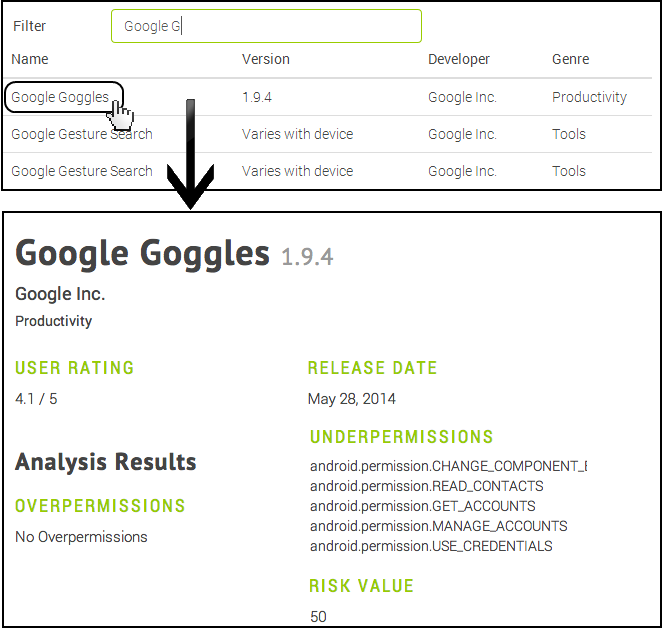
\includegraphics[width=\columnwidth, angle = 0]{images/screenshot3.png}
\caption{\ifisnopii darwin.rit.edu \else xxx.hidden.edu \fi Website Reporting Tool}
\label{fig:website1}
\end{figure}


 \begin{figure}[ht!]
\centering
%\frame{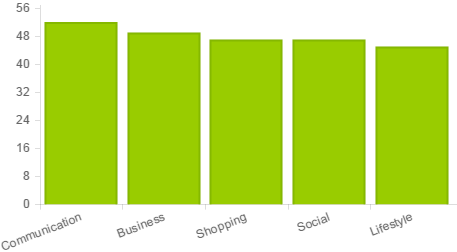
\includegraphics[scale=.5]{images/overprivsByGenre.png}}
%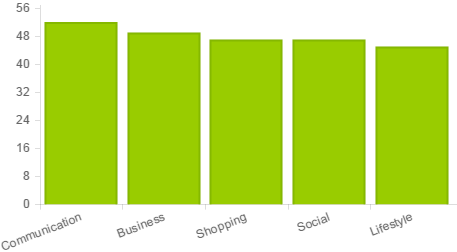
\includegraphics[scale=.7]{images/overprivsByGenre.png}
 \par\framebox[1.1\width]{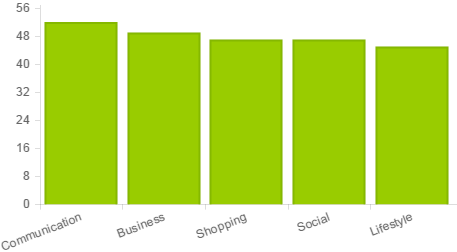
\includegraphics[scale=.63]{images/overprivsByGenre.png}}
\caption{Overprivileged Apps By Genre from Project Website}
\label{fig:overprivappsByGenre}
\end{figure}


%The website also includes several data driven result sets about apps at a more aggregate level. Figure~\ref{fig:overprivappsByGenre} shows an example graph with the percentage of apps in the top 5 genres which contain at least 1 overprivilege.

The website also includes several data driven result sets about apps at a more aggregate level. One example is shown in Figure~\ref{fig:overprivappsByGenre}, which displays an example graph with the percentage of apps in the top 5 genres which contain at least 1 overprivilege.




% http://darwin.rit.edu/reports
16 prebuilt reports in .csv format are available in several areas including the rate at which two overprivileges appear together in all applications, the percentage of times each overprivilege occurs in all applications, and the percentage of times each overprivilege occurs in all applications.





\section{Limitations \& Future Work}
\label{sec:limitations}


While static analysis tools have demonstrated their value in numerous previous works~\cite{Felt:2011:APD:2046707.2046779, Pearce:2012:APS:2414456.2414498}, it is unreasonable to expect that any tool will ever be flawless and that no static analysis tool is perfect and generally inherently contains limitations~\cite{chess2004static}. Although Stowaway is a powerful static analysis tool which has been used in previous research~\cite{Pearce:2012:APS:2414456.2414498,Stevens_investigatinguser,jeon2011dr}, it does suffer from drawbacks. Stowaway's own authors state that the tool only achieves 85\% code coverage~\cite{Felt:2011:APD:2046707.2046779}, so the over \& under privileges reported by this tool are imperfect. Additionally, any reported vulnerabilities or defects by a static analysis tool should be deemed as~\emph{possible} vulnerabilities or defects, not necessarily actual ones.

Identifying possible vulnerabilities or security risks is extremely difficult, and like any static analysis tool AndroRisk is only capable of making educated observations about the risk level of an app and that more substantial risk assessments will require a far more substantial level of analysis, which will likely include a manual investigation of the app. Due to the large number of examined apps in our study, this thorough level of analysis was not practical. Even with almost certain imperfections, we believe that AndroRisk was a good choice due to its ability to quickly analyze apps and its use in existing research~\cite{krutz2015FDroid}.

We compiled much of our data through reverse engineering APK files from the Google Play store. While similar reverse engineering techniques have been successfully used in previous works~\cite{Lee_2013,6687155}, no reverse engineering process can ever be expected to be totally accurate. However, based on manually verifying a small subset of our results and previous research, we have a high confidence in our reverse engineering process.


%We only analyzed apps from Google Play and not other sources such as AppksAPK or F-Droid, which would have led to more varied application origins. However, we feel the diversity of our apps was already quite robust since we collected 70,785  applications from 41 genres. %We also only examined free applications in our research due to cost constrains. Thus, the measurements comparison of apps is not representative of the entire Google Play market. Our results only apply as an evaluation of free apps, not paid apps.


While we have demonstrated profound results through the collection of over 70,000 Android apps, future work may be conducted in several key areas. We only analyzed free apps, and an interesting study would be to compare the free and paid apps using a similar process as ours. Future studies could also analyze how apps evolve over time through the examination of numerous released versions of the same app. Google's new API ``M'', received a massive permissions overhaul and work may be done to see how this new release affects how developers use permissions. Naturally more apps can always be examined, and with new apps being released on a daily basis the process is never ending. Additional research may also be done to examine apps collected from other sources, such as AppksAPK or F-Droid.


%   ? Adoption rates of new Android APis    - Might not be a great idea to include this
%   Further undestanding of what these values mean
%   Website enhancements


%%  What was said in evaluations that we can address here




\section{Conclusion}
\label{sec: conclusion}

In this work, we described our process of gathering and analyzing 70,785 Android applications in a variety of areas including security vulnerability level, overprivileges, code clones, potential defects, and coding standards mistakes.
 We also provide a robust dataset and website which may be used by future researchers in their work.


%We found that, on average, Android applications increase in their potential security risks with each release while increase instances of code clones and decreasing potential defects. We conducted our analysis within genres and found that certain genres included more instances of overprivileges. As a control, we compared our analysis results against known malware and found that the static analysis tools we employed demonstrated high levels of security risk where malware was known. These results provide a broad overview of the state of the breadth of free apps in the Google Play store.

%\section*{Acknowledgment}

%This research would not have been possible without the hard work by two dedicated Software Engineering Students: Shannon Trudeau and Adam Blaine. We would like to thank them for their dedication and the insights they have provided on this project.


\section*{Acknowledgements}

\ifisnopii % turn on/off pii
% Meiyappan Nagappan
\todo{put information in here}
\else % turn on/off pii
Author and funding acknowledgments hidden for review anonymity.
\fi % end turn on/off pii


\balance
\bibliographystyle{abbrv}
\bibliography{AndroidData}



% That's all folks!
\end{document}




%%%% Submission location
% 	Confirmation Number:	1071
%	Submission Passcode:	1071X-F3B7P9G7F8

% https://www.softconf.com/f/sac2016/cgi-bin/scmd.cgi?scmd=aLogin&passcode=1071X-F3B7P9G7F8



%   Due date: September 11, 2015 - http://selab.uos.ac.kr/sacse16/
%   SQL Queries located at: https://docs.google.com/document/d/1-z0AsZFgbz8UF2j0eLyw5Tp7YhJFczjARBgrwebqURw/edit

%   	Take into account ICSE feedback
%   	Make sure keywords and formatting is all set
%   	Use the term "overprivilege" & "Google_Play"
%   Make sure "Blind" version of paper hides all identifiable info and proofread with that info

% Think about doing a MWU analysis? - not sure if this would be applicable for any areas of the app.

% &&&&&&&&&&&&&&&&&

%   What comments were made about the SAC papers that did not get in last year?
%   Fix citations. I think some of the citations to the URLs could be made better.
%   Add in a small section for Recommendations - How could these problems be solved by developers
%   ? Add SQL query window onto webpage ?
%       Would need to speak with Jared about this
%   Make sure it is "AndroRisk" - case sensitive
%   Should the security and other aspects of the paper be separated out?




% &&&&&&&&&&&&&&&&&
%% What correlations exist between static analysis metrics and apps- reword
%% 		How do genres compare to one another
%% 		LIfecycle of apps - by release date
%% 		Is there a general correlation among metrics
%% 		Do quality metrics change between apps with more or less than 10K downloads




% How pervasive are overpriviledge in Android apps - reword this
%% 		What are the most pervasive overprivileges?
%% 		Where there is one overpriviledge, are there more



%%%%% Make sure to provide some analysis with these



%%%%% Other RQs
%	Do developers make use of new Android permissions?
%	Do people use new API versions?
%   	Would need to hook this into dates as well. Demonstrate that apps were able to swtich APIs
%	Look at the lifecycle of apps based on their release date. How are things changing?





% Interesting paper - PlayDrone
%   http://engineering.columbia.edu/columbia-engineering-team-finds-thousands-secret-keys-android-apps-0


